\documentclass[dvipdfmx]{jarticle}
\usepackage{graphicx}
\usepackage[top=30truemm,bottom=30truemm,left=25truemm,right=25truemm]{geometry}
\usepackage{listings,jvlisting}
\usepackage{url}
\usepackage{tikz}
\usetikzlibrary{arrows.meta, positioning, automata}

\lstset{
  basicstyle={\ttfamily},
  identifierstyle={\small},
  commentstyle={\smallitshape},
  keywordstyle={\small\bfseries},
  ndkeywordstyle={\small},
  stringstyle={\small\ttfamily},
  frame={tb},
  breaklines=true,
  columns=[l]{fullflexible},
  numbers=left,
  xrightmargin=0zw,
  xleftmargin=3zw,
  numberstyle={\scriptsize},
  stepnumber=1,
  numbersep=1zw,
  lineskip=-0.5ex
}

\begin{document}
\begin{titlepage}
    \begin{center}
        {\huge 情報科学実験B 課題2レポ―ト}
        \vspace{180pt}\\
        \begin{tabular}{rl}
            氏名 & 山久保孝亮\\
            所属 & 大阪大学基礎工学部情報科学科ソフトウェア科学コース\\
            メールアドレス & u327468b@ecs.osaka-u.ac.jp\\
            学籍番号 & 09B22084\\
            提出日 & \today\\
            担当教員 & 小南大智,松本麻佑
        \end{tabular}
    \end{center}
\end{titlepage}
\section{システムの仕様}
今回の課題で作成した私の電卓の仕様は以下の通りである.
\begin{itemize}
    \item 二つの数値の四則演算を実行する.即ち,1+2のような計算を実行する.今回の課題では1+1+1のような3つ以上の数値の計算には対応していない.
    \item 初期状態では7セグメントデコーダは全消灯している.また,今回の電卓では回路上でHIGHかLOWかを決める4つの入力があり,その4つの入力を操作してからスイッチを開放したときにのみ出力が変化する.
    \item 0から9が入力されるとそのままの数値が,10から13が入力されると小さい順に+,-,*,/が入力されたと考える.15を入力しスイッチを開放すると結果を計算し,もう一度スイッチを開放すると結果を表示する.
    \item 入力する際の二つの数値は複数桁にも対応している.例えば1と2を連続で入力した際には12という数値を表すようにした.また,桁数は最大3桁で4桁以上の数値が入力すなわち4回以上連続で数値が入力された場合は
    エラーとする.また,01のように数値を入力した際は1を数値として考えるが,0001のように4つ以上の数値が入力された場合は前述の仕様により,エラーとする.
    \item 計算結果は15を入力してスイッチを開放してから再びスイッチを開放したときに表示される.計算結果が複数桁の際にはスイッチ解放の度に上位桁から順番に表示する.全ての桁を出力してから再びスイッチを開放したときに初期状態に戻る.
    \item エラー処理は7セグメントLEDに入力が14のときの出力を1秒間表示させた後に初期状態に戻る.
    \item 引き算において計算結果が負の数になった場合は絶対値となって答えを出力する.即ち,1-4を実行すると-3ではなく3を出力するという仕様である.また,割り算において0で割った際はエラーとなる.
    \item 数値,演算子,数値の形に従わない数式が入力された場合はエラーが表示される.
\end{itemize}
\section{ハードウェア回路}
今回の電卓の課題ではプッシュスイッチの制御回路,7セグメントLEDの制御回路,Arduinoの入力と出力をつなぐ回路を実現した.
以下でこれらの詳細について順に述べる.
\begin{enumerate}
    \item プッシュスイッチの制御回路は以下の図1の指導書にあったチャタリング防止付きの回路を実装した.\cite{1}
    この回路は以下の図2のように,スイッチが上のような挙動ではなく下のような挙動になってしまうことを防ぐものである.\cite{2}
    
    \begin{figure}[h]
        \begin{minipage}[b]{0.45\linewidth}
          \centering
          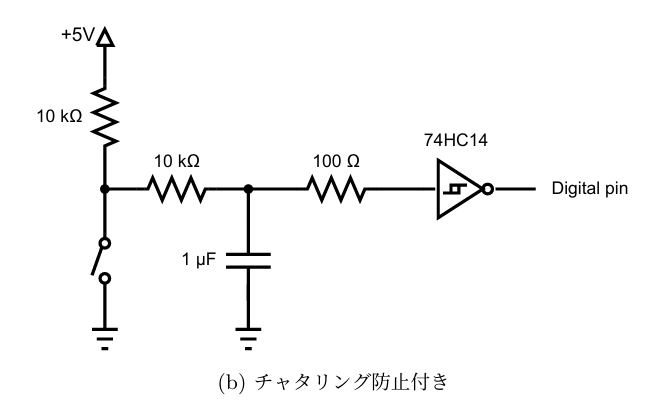
\includegraphics[keepaspectratio, scale=0.4]{tyataringu.png}
          \caption{チャタリング防止回路}
        \end{minipage}
        \begin{minipage}[b]{0.45\linewidth}
          \centering
          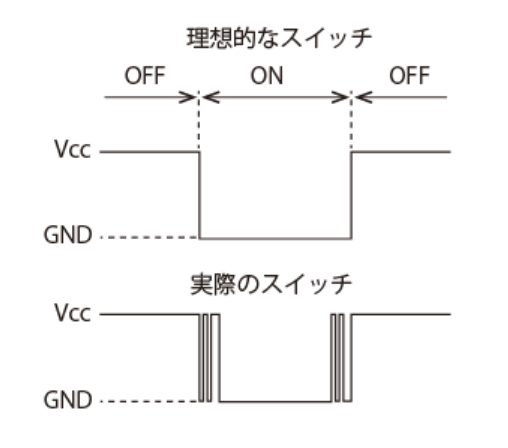
\includegraphics[keepaspectratio, scale=0.4]{switch.png}
          \caption{スイッチの様子}
        \end{minipage}
      \end{figure}
      チャタリング防止回路はコンデンサにたまった電荷が急に変化しないという性質を利用して,チャタリングによってスイッチのオンオフが繰り返し行われたとしても,実際の電圧の変化はコンデンサの電荷の減少に従うようにして影響を受けないようにしたものである.コンデンサの左側二つの抵抗はこの電荷の減少の速さを抑えて影響を受けない時間を長くするという目的のため置かれている.
    ただし,コンデンサによって電圧がHIGHとLOWの中間の値をとってしまうので,その中間地をHIGHとLOWに再び分類するためにシュミットトリガ・NOTが置かれている.その直前の抵抗は,シュミットトリガ・NOTの電源電圧の最大値が6Vであることから,電圧の値を下げるということが目的であると考えられる.\cite{3}そして図1のDigital pinをArduinoの指定したピンにつなぐ.(私の場合はピン8)
    \item 7セグメントLEDの制御は以下の図3の7447デコーダのaからgに対応するピンを図4のLEDの対応するピンにつなぐことで実現した.\cite{1}
    \begin{figure}[h]
        \begin{minipage}[b]{0.45\linewidth}
          \centering
          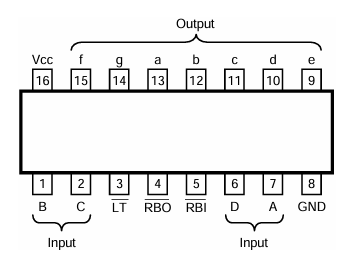
\includegraphics[keepaspectratio, scale=0.4]{7447.png}
          \caption{7447デコーダ}
        \end{minipage}
        \begin{minipage}[b]{0.45\linewidth}
          \centering
          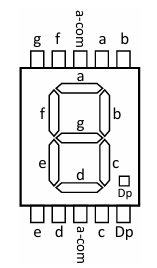
\includegraphics[keepaspectratio, scale=0.4]{7seg.png}
          \caption{7セグメントLED}
        \end{minipage}
      \end{figure}\\
    \item 7447デコーダのAからDに対応するピンには,arduino内部で処理した後の出力を与えるので指定したピンとつないだ.(私の場合はピン4\~ピン7)arduinoへの入力は5Vまたはグラウンドにつないだ線をarduinoの指定したピンに差し込んだ.(私の場合はピン9\~ピン12)
\end{enumerate}
\section{制御プログラム}
私が作成した電卓の制御プログラムの状態遷移図は以下のようになる.\\\\
\begin{center}
    \begin{tikzpicture}[->, >=Stealth, node distance=4cm, on grid, auto,
        state/.style={circle, draw, minimum size=1.5cm, inner sep=0pt}]
    
      % States
      \node[state] (start) {開始};
      \node[state, right=of start] (readInput) {入力読取};
      \node[state, right=of readInput] (processInput) {入力処理};
      \node[state, right=of processInput] (calculate) {計算};
      \node[state, below=2cm of processInput] (output) {結果出力};
      \node[state, below=2cm of readInput] (error) {エラー処理};
    
      % Initial State Arrow
      \node[below=0.75cm of start] (initial) {};
      \path[->, >=Stealth] (initial) edge (start);
    
      % State Transitions
      \path[every node/.style={font=\sffamily\small}]
        (start) edge node[above] {セットアップ} (readInput)
        (readInput) edge [loop above] node {入力待ち} (readInput)
        (readInput) edge [bend left] node[above, pos=0.5] {ボタン押下} (processInput)
        (processInput) edge node[above, pos=0.5] {入力確認} (calculate)
        (calculate) edge [bend left] node[below, pos=0.5] {有効入力} (output)
        (error) edge [loop below] node {エラー表示} (error)
        (error) edge node[left, pos=0.5] {リセット} (readInput)
        (output) edge [bend right=45, above] node[above, pos=0.5] {表示完了} (readInput);
    
      % Additional Transitions for Handling Errors and Calculations
      \path[blue]
        (processInput) edge [bend right] (error)
        (calculate) edge [bend right] (error);
    
    \end{tikzpicture}
    \end{center}
    青色の有効辺はエラー処理に向かう有効辺である.エラー処理,入力処理,計算,結果出力はそれぞれ関数として表現し,デバッグを行いやすくした.また,状態遷移はスイッチが解放された瞬間のみに行われるという機能を実装するためにchangeという変数を用意し,スイッチが解放されたときにのみchangeが1に,それ以外では0という条件分岐を実現することで非トラッキング回路で実現した.
    また,数式の記憶は要素数7個の配列memoryを,表示する計算結果の記憶は要素数6個の配列answer\_memoryをそれぞれグローバル変数として使用した.
    以下では,上記の関数とloop関数の実装について記述する.
    \subsection{loop関数}
    loop関数ではまずエラーが起きたかどうか(error\_flag)を判定する.error\_flagが1であれば後述のerror関数を呼び出して終了する.1でなければ,スイッチを開放したかどうか(change)のフラグを判定する.スイッチが解放された瞬間を検出するために,直前にスイッチが押されていたかどうかを記憶する変数previousbuttonStateと現在のスイッチの状態を表すbuttonStateを使用する.直前は押していて,現在は押していない即ちpreviousbuttonStateが1でbuttonStateが0となった際にchangeを1に変更する.
    changeが1でなければ,loop関数を終了する.changeが1であれば,changeを0に戻して結果を出力するかどうか(answer\_flag)のフラグを判定する.1であれば,後述のoutput関数で結果を出力する.1でなければ,二進数の4つの入力を十進数に変換してsumに格納する.sumの値によって条件分岐する.sumが15であれば3.3で述べるcombine関数によって入力処理を行う.このとき,入力処理が正常に終了すれば計算式が記憶されている配列の1番目の要素には
    演算子に相当する数値が格納され,4番目以降はすべて-1になるという仕様にしたため,条件分岐でそれらを判定し,3.4で述べる計算処理を実行する.sumの値が15以外ならばmemoryに入力した数式を格納していく.数値を入力していくたびにinput\_counterを1増やし,7セグメントLEDを入力した数値に光らせる.今回の仕様上三桁と三桁の四則演算が最大の入力数になるので入力した数値が8個になると強制的にエラーのフラグを立てる.
    \subsection{エラー処理}
    1で述べた仕様のように,エラーが起きる可能性のある所に条件分岐を作り,millis関数で現在の時間を取得してグローバル変数nowに格納し,error\_flagを1にする.そうすることで,loop関数の最初の条件分岐でerror関数を呼び出しすことができる.これは非トラッキング処理を
    エラー関数ではエラー関数内で再びmillis関数を呼び出してエラーが発生した段階の時間を格納しているnowとの差が1000以下の時,つまりエラーが発生してから1秒以下の時は7セグメントLEDに14を表示させる.1秒経つと全消灯にして使用しているグローバル変数の初期化を行う.
    \subsection{入力処理}
    0から始まるカウンタiをinput\_counterの値と等しくなるまでwhile文を実行する.while文の内容は,まずmemory[i]の値が10未満かどうかを判定し,i番目に格納されているものが数値であるのか演算子であるのかを判定する.そして,数値であれば
    memory[i+1]が10未満かどうかを判定する.これにより,21のような二桁の数値が入力されたときの条件分岐を作成した.同様にしてmemory[i+2]を判定して三桁の数値の時の条件分岐を作成した.2桁であったときにはmemory[i]にmemory[i]を10倍したものとmemory[i+1]を足し合わせたものを格納しmemory全体を一つずつ左に寄せる.同様に,3桁であったときにはmemory[i]にmemory[i]を百倍したものとmemory[i+1]を10倍したものとmemory[i+2]を足し合わせたものを格納しmemory全体を二つ左に寄せる.これらはinput\_counterの値を超えない範囲で行われる.
    また,左にずらした分だけinput\_counterの値も減らされる.そしてwhile文が終了した後にmemoryのinput\_counterの値のインデックスから最後まで-1が格納される.これによりloop関数での入力処理が正しく行われたかどうかを条件分岐で正常に判定することができる.-1を選んだ理由は,どのように入力をしても負の値を入力することはできないからである.
    \subsection{計算}
    3.3の入力処理により,memoryには順に数値,演算子,数値が格納されているはずなので,memory[1]の値によってどの演算を実行するかを判定して計算結果をlong型変数answerに格納した.
    今回の仕様では数値は三桁までなのでanswerがとりうる最大の値は999*999=998001だが,int型を使うと32767以上の値はオーバーフローをしてしまうのでlong型を使用した.引き算は仕様により絶対値で表すのでabs関数を利用した.掛け算ではmemory[0]とmemory[1]をlong型に型変換して計算した.
    そしてanswerの値をtempという変数にコピーし、10で何回割ることができるかを確認する.これにより,計算結果が何桁であるのかを調べることができる.そして10で割った余りをanswer\_memoryに格納する.
    
    \subsection{結果出力}
    結果を出力するのはスイッチを開放した瞬間であるため,answerフラグを立ててoutput関数をloopすることができるようにした.output関数では最初に表示した回数を数えるcountが桁数未満かどうかを判定する.条件式が真であればanswer\_memory[count]の数値を二進数に変換し7セグメントLEDに表示させてcountの値を1増やす.偽であればanswer\_flagを0にして7セグメントLEDを全消灯にしてmemoryやanswer\_memoryを初期化する.
\section{考察と工夫点}
今回私が電卓を実装するにあたって工夫した点はエラーが発生した際に自動で初期状態に復帰するようにした点である.7セグメントLEDを14の値のままで光らせ続けると,エラー処理によって光っているのか何らかのプログラムのミスによって14として光っているのかを判別できる.また,エラーが発生するのは数式を間違って入力したときであるため,直後に
正しい数式を入力する可能性が高いので初期状態に戻ることで素早く次の操作に移ることができる.考察としては,この工夫点の拡張として数式を入力している途中にエラーであることが確定した場合にエラーとする処理を追加することである.この場合はエラーを表示している途中にユーザが気づかずに数式を入力する可能性があるのでエラーを表示している間は入力を受け付けないようにするなどの機能が必要である.
\section{感想}
今回の電卓の課題を実装して感じたことは,ループ関数があるときにはフラグを使うと設計がしやすいということである.フラグを使うことによって自然に非トラッキング処理を実装することができた.
\section{謝辞}
本課題を実装するにあたって講義時間中の質問応答や動作確認などのご協力をしていただき有難うございました.今後の課題3,4とも宜しくお願いいたします.
\begin{thebibliography}{10}
    \bibitem{1} 情報科学実験B指導書
    \bibitem{2} \url{https://www.marutsu.co.jp/pc/static/large_order/1405_311_ph} 2024/05/16アクセス
    \bibitem{3} \url{https://akizukidenshi.com/catalog/g/g110923/} 2024/05/16 アクセス
\end{thebibliography}
\end{document}